\documentclass{ximera}

\usepackage{epsfig}

\graphicspath{
  {./}
  {figures/}
}

\usepackage{epstopdf}
%\usepackage{ulem}
\usepackage[normalem]{ulem}

\epstopdfsetup{outdir=./}

\usepackage{morewrites}
\makeatletter
\newcommand\subfile[1]{%
\renewcommand{\input}[1]{}%
\begingroup\skip@preamble\otherinput{#1}\endgroup\par\vspace{\topsep}
\let\input\otherinput}
\makeatother

\newcommand{\EXER}{}
\newcommand{\includeexercises}{\EXER\directlua{dofile(kpse.find_file("exercises","lua"))}}

\newenvironment{computerExercise}{\begin{exercise}}{\end{exercise}}

%\newcounter{ccounter}
%\setcounter{ccounter}{1}
%\newcommand{\Chapter}[1]{\setcounter{chapter}{\arabic{ccounter}}\chapter{#1}\addtocounter{ccounter}{1}}

%\newcommand{\section}[1]{\section{#1}\setcounter{thm}{0}\setcounter{equation}{0}}

%\renewcommand{\theequation}{\arabic{chapter}.\arabic{section}.\arabic{equation}}
%\renewcommand{\thefigure}{\arabic{chapter}.\arabic{figure}}
%\renewcommand{\thetable}{\arabic{chapter}.\arabic{table}}

%\newcommand{\Sec}[2]{\section{#1}\markright{\arabic{ccounter}.\arabic{section}.#2}\setcounter{equation}{0}\setcounter{thm}{0}\setcounter{figure}{0}}
  
\newcommand{\Sec}[2]{\section{#1}}

\setcounter{secnumdepth}{2}
%\setcounter{secnumdepth}{1} 

%\newcounter{THM}
%\renewcommand{\theTHM}{\arabic{chapter}.\arabic{section}}

\newcommand{\trademark}{{R\!\!\!\!\!\bigcirc}}
%\newtheorem{exercise}{}

\newcommand{\dfield}{{\sf SlopeField}}

\newcommand{\pplane}{{\sf PhasePlane}}

\newcommand{\PPLANE}{{\sf PHASEPLANE}}

% BADBAD: \newcommand{\Bbb}{\bf}. % Package amsfonts Warning: Obsolete command \Bbb; \mathbb should be used instead.

\newcommand{\R}{\mbox{$\mathbb{R}$}}
\let\C\relax
\newcommand{\C}{\mbox{$\mathbb{C}$}}
\newcommand{\Z}{\mbox{$\mathbb{Z}$}}
\newcommand{\N}{\mbox{$\mathbb{N}$}}
\newcommand{\D}{\mbox{{\bf D}}}

\newcommand{\WW}{\mathcal{W}}

\usepackage{amssymb}
%\newcommand{\qed}{\hfill\mbox{\raggedright$\square$} \vspace{1ex}}
%\newcommand{\proof}{\noindent {\bf Proof:} \hspace{0.1in}}

\newcommand{\setmin}{\;\mbox{--}\;}
\newcommand{\Matlab}{{M\small{AT\-LAB}} }
\newcommand{\Matlabp}{{M\small{AT\-LAB}}}
\newcommand{\computer}{\Matlab Instructions}
\renewcommand{\computer}{M\small{ATLAB} Instructions}
\newcommand{\half}{\mbox{$\frac{1}{2}$}}
\newcommand{\compose}{\raisebox{.15ex}{\mbox{{\scriptsize$\circ$}}}}
\newcommand{\AND}{\quad\mbox{and}\quad}
\newcommand{\vect}[2]{\left(\begin{array}{c} #1_1 \\ \vdots \\
 #1_{#2}\end{array}\right)}
\newcommand{\mattwo}[4]{\left(\begin{array}{rr} #1 & #2\\ #3
&#4\end{array}\right)}
\newcommand{\mattwoc}[4]{\left(\begin{array}{cc} #1 & #2\\ #3
&#4\end{array}\right)}
\newcommand{\vectwo}[2]{\left(\begin{array}{r} #1 \\ #2\end{array}\right)}
\newcommand{\vectwoc}[2]{\left(\begin{array}{c} #1 \\ #2\end{array}\right)}

\newcommand{\ignore}[1]{}


\newcommand{\inv}{^{-1}}
\newcommand{\CC}{{\cal C}}
\newcommand{\CCone}{\CC^1}
\newcommand{\Span}{{\rm span}}
\newcommand{\rank}{{\rm rank}}
\newcommand{\trace}{{\rm tr}}
\newcommand{\RE}{{\rm Re}}
\newcommand{\IM}{{\rm Im}}
\newcommand{\nulls}{{\rm null\;space}}

\newcommand{\dps}{\displaystyle}
\newcommand{\arraystart}{\renewcommand{\arraystretch}{1.8}}
\newcommand{\arrayfinish}{\renewcommand{\arraystretch}{1.2}}
\newcommand{\Start}[1]{\vspace{0.08in}\noindent {\bf Section~\ref{#1}}}
\newcommand{\exer}[1]{\noindent {\bf \ref{#1}}}
\newcommand{\ans}{\textbf{Answer:} }
\newcommand{\matthree}[9]{\left(\begin{array}{rrr} #1 & #2 & #3 \\ #4 & #5 & #6
\\ #7 & #8 & #9\end{array}\right)}
\newcommand{\cvectwo}[2]{\left(\begin{array}{c} #1 \\ #2\end{array}\right)}
\newcommand{\cmatthree}[9]{\left(\begin{array}{ccc} #1 & #2 & #3 \\ #4 & #5 &
#6 \\ #7 & #8 & #9\end{array}\right)}
\newcommand{\vecthree}[3]{\left(\begin{array}{r} #1 \\ #2 \\
#3\end{array}\right)}
\newcommand{\cvecthree}[3]{\left(\begin{array}{c} #1 \\ #2 \\
#3\end{array}\right)}
\newcommand{\cmattwo}[4]{\left(\begin{array}{cc} #1 & #2\\ #3
&#4\end{array}\right)}

\newcommand{\Matrix}[1]{\ensuremath{\left(\begin{array}{rrrrrrrrrrrrrrrrrr} #1 \end{array}\right)}}

\newcommand{\Matrixc}[1]{\ensuremath{\left(\begin{array}{cccccccccccc} #1 \end{array}\right)}}



\renewcommand{\labelenumi}{\theenumi}
\newenvironment{enumeratea}%
{\begingroup
 \renewcommand{\theenumi}{\alph{enumi}}
 \renewcommand{\labelenumi}{(\theenumi)}
 \begin{enumerate}}
 {\end{enumerate}
 \endgroup}

\newcounter{help}
\renewcommand{\thehelp}{\thesection.\arabic{equation}}

%\newenvironment{equation*}%
%{\renewcommand\endequation{\eqno (\theequation)* $$}%
%   \begin{equation}}%
%   {\end{equation}\renewcommand\endequation{\eqno \@eqnnum
%$$\global\@ignoretrue}}

%\input{psfig.tex}

\author{Martin Golubitsky and Michael Dellnitz}

%\newenvironment{matlabEquation}%
%{\renewcommand\endequation{\eqno (\theequation*) $$}%
%   \begin{equation}}%
%   {\end{equation}\renewcommand\endequation{\eqno \@eqnnum
% $$\global\@ignoretrue}}

\newcommand{\soln}{\textbf{Solution:} }
\newcommand{\exercap}[1]{\centerline{Figure~\ref{#1}}}
\newcommand{\exercaptwo}[1]{\centerline{Figure~\ref{#1}a\hspace{2.1in}
Figure~\ref{#1}b}}
\newcommand{\exercapthree}[1]{\centerline{Figure~\ref{#1}a\hspace{1.2in}
Figure~\ref{#1}b\hspace{1.2in}Figure~\ref{#1}c}}
\newcommand{\para}{\hspace{0.4in}}

\usepackage{ifluatex}
\ifluatex
\ifcsname displaysolutions\endcsname%
\else
\renewenvironment{solution}{\suppress}{\endsuppress}
\fi
\else
\renewenvironment{solution}{}{}
\fi

\ifcsname answer\endcsname
\renewcommand{\answer}{}
\fi

%\ifxake
%\newenvironment{matlabEquation}{\begin{equation}}{\end{equation}}
%\else
\newenvironment{matlabEquation}%
{\let\oldtheequation\theequation\renewcommand{\theequation}{\oldtheequation*}\begin{equation}}%
  {\end{equation}\let\theequation\oldtheequation}
%\fi

\makeatother

\newcommand{\RED}[1]{{\color{red}{#1}}} 


\title{Coupled Linear Systems}

\begin{document}
\begin{abstract}
\end{abstract}
\maketitle

 \index{coupled system} 
 \label{s:3.5}


The general linear constant coefficient system in two unknown functions 
$x_1,x_2$ is:
\renewcommand{\arraystretch}{1.8}
\begin{equation}\label{lin3}
\begin{array}{ccc}
\dps \frac{dx_1}{dt}(t) & = & ax_1(t) + bx_2(t) \\
\dps \frac{dx_2}{dt}(t) & = & cx_1(t) + dx_2(t).
\end{array}
\end{equation}
\renewcommand{\arraystretch}{1.0}%
The uncoupled systems studied in Section~\ref{sec:UncoupledLS} are obtained 
by setting $b=c=0$ in \eqref{lin3}.  We have discussed how to solve \eqref{lin3} 
by formula \eqref{e:explicitsoln} when the system is uncoupled.  We have also 
discussed how to visualize the phase plane for different choices of the 
diagonal entries $a$ and $d$.  At present, we cannot
solve \eqref{lin3} by formula when the coefficient matrix is not diagonal.
But we may use {\pplane} to solve the initial value problems numerically 
for these coupled systems.  We illustrate this point by solving
\begin{eqnarray*}
\frac{dx_1}{dt}(t) & = &  -x_1(t) + 3x_2(t) \\
\frac{dx_2}{dt}(t) & = &  3x_1(t) - x_2(t).
\end{eqnarray*}
After starting {\pplane}, select {\sf linear system} from the
{\sf Gallery} and set the constants to:
\[
	a = -1,\quad b = 3,\quad c = 3, \quad d = -1.
\]
In order to have equally spaced coordinates on
the $x$ and $y$ axes, do the following.   In the \pplane\; {\sf Display} 
window enter $x_0 = 0.5$ and $y_0 = 0$ and click on {\sf Update}.
Repeat three times with $x_0 = -0.5$ and $y_0 = 0$, $x_0 = 0$ and $y_0 = 0.5$, 
and $x_0 = 0$ and $y_0 = -0.5$ to recreate Figure~\ref{F:invariantlines}.

\subsection*{Eigendirections}

After computing several solutions, we find that for increasing
time $t$ all the solutions seem to approach the diagonal line
given by the equation $x_1=x_2$. Similarly, in backward time $t$
the solutions approach the anti-diagonal $x_1=-x_2$.  In other
words, as for the case of uncoupled systems, we find two
distinguished directions in the $(x,y)$-plane.  See
Figure~\ref{F:invariantlines}.  Moreover, the computations
indicate that these lines are invariant in the sense that
solutions starting on these lines remain on them for all time.
This statement can be verified numerically by choosing initial
conditions $(x_0,y_0)=(1,1)$ and $(x_0,y_0)=(1,-1)$.

\begin{figure}[htb]
     \centerline{%
     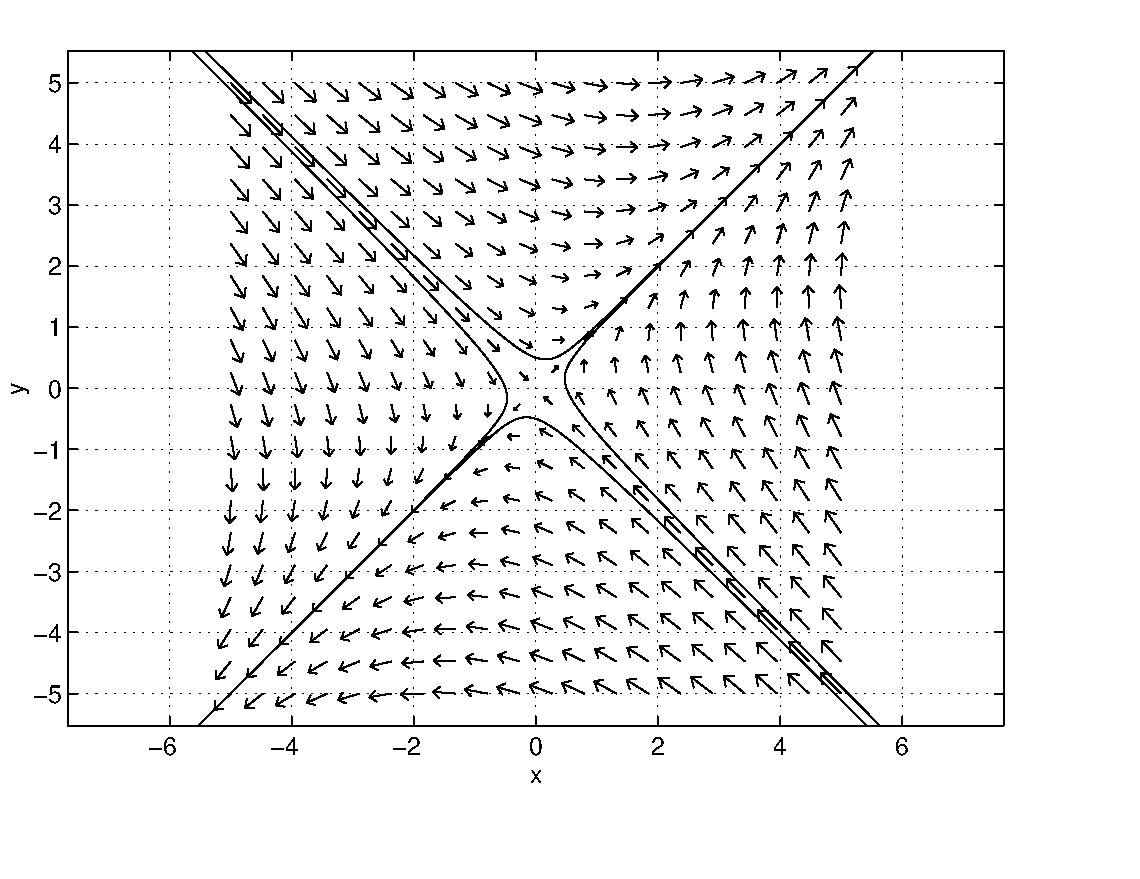
\includegraphics[width=3.5in]{../figures/invline.pdf}}
     \caption{{\sf \PPLANE\ Display} for \protect\eqref{lin3} with
             $a=-1=d$; $b=3=c$; and $x,y\in [-5,5]$.
	Solutions going through $(\pm 0.5,0)$ and $(0,\pm 0.5)$ are shown.}
     \label{F:invariantlines}
\end{figure}

\begin{definition} \label{D:eigendirection}
An invariant line for a linear system of differential equations
is called an {\em eigendirection}\index{eigendirection}.
\end{definition}

Observe that eigendirections vary if we change parameters.  For
example, if we set $b$ to $1$, then there are still two
distinguished lines but these lines are no longer perpendicular.

For uncoupled systems, we have shown analytically that the $x$
and $y$ axes are eigendirections.  The numerical computations
that we have just performed indicate that eigendirections exist
for many coupled systems.  This discussion leads naturally to
two questions:
\begin{enumerate}
\item Do eigendirections always exist?
\item How can we find eigendirections?
\end{enumerate}
The second question will be answered in Sections~\ref{S:IVP&E} and 
\ref{S:evchp}.  We can answer the first question by performing another 
numerical computation.  In the setup window, change the parameter $b$ 
to $-2$.  Then numerically compute some solutions to see that there
are no eigendirections in the phase space of this system.  Observe that
all solutions appear to spiral into the origin as time goes to
infinity.  The phase portrait is shown in Figure~\ref{pp_dsp2}.
\begin{figure}[htb]
      \centerline{%
      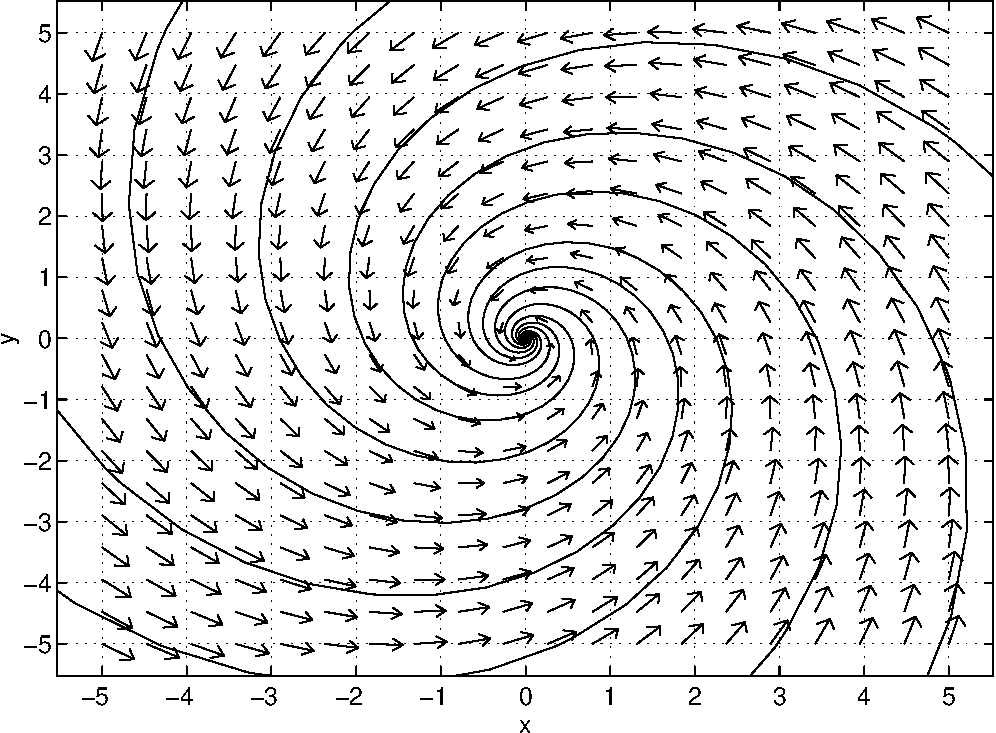
\includegraphics[width=3.5in]{../figures/pp_dsp2.pdf}}
      \caption{{\sf \PPLANE\ Display} for the {\sf linear system}
		with $a=-1$, $b=-2$, $c=3$, $d=-1$.}
      \label{pp_dsp2}
\end{figure}


\subsubsection*{Nonexistence of Eigendirections}

We now show analytically that certain linear systems of
differential equations have no invariant lines in their phase portrait.
Consider the system
\begin{equation}  \label{E:2nd->1st}
\begin{array}{rcl}
\dot{x} & = & y \\
\dot{y} & = & -x.
\end{array}
\end{equation}
Observe that $(x(t),y(t))=(\sin t, \cos t)$ is a solution to \eqref{E:2nd->1st} by calculating
\[
\begin{array}{rclcrcr}
\dot x(t) & = & \frac{d}{dt} \sin t & = & \cos t & = & y(t)\\
\dot y(t) & = & \frac{d}{dt} \cos t&  = & -\sin t & = & -x(t)
\end{array}
\]
We have shown analytically that the unit circle centered at the origin is a solution 
trajectory for \eqref{E:2nd->1st}.  Hence \eqref{E:2nd->1st} has no 
eigendirections.  It may be checked using \Matlab that all solution 
trajectories for \eqref{E:2nd->1st} are just circles centered at the origin.




\includeexercises


\end{document}
